% !TeX Options = -shell-escape
\documentclass{panicsoftware-presentation}

\usepackage{tikz}
\usetikzlibrary{decorations.pathreplacing}

\title{Lifetime of the C++ object?}
\author{Dawid Pilarski}
\date{}

\institute{dawid.pilarski@tomtom.com \\ dawid.pilarski@panicsoftware.com \\ \href{http://blog.panicsoftware.com}{blog.panicsoftware.com} }

\newenvironment{itemizeSeq}{\begin{itemize}[<+-|alert@+>]}{\end{itemize}}
\newenvironment{itemizeNColorSeq}{\begin{itemize}[<+->]}{\end{itemize}}

\begin{document}

\begin{frame}
	\maketitle
\end{frame}

\section*{Introduction}

\begin{frame}{Agenda}
	\tableofcontents
\end{frame}

\begin{frame}{Who am I?}

\end{frame}

\begin{frame}{Questions.}
	
	\vfill
	\centerline{Questions...}
	\vfill

\end{frame}

\begin{frame}{What we talk about are basics.}

	\centering
	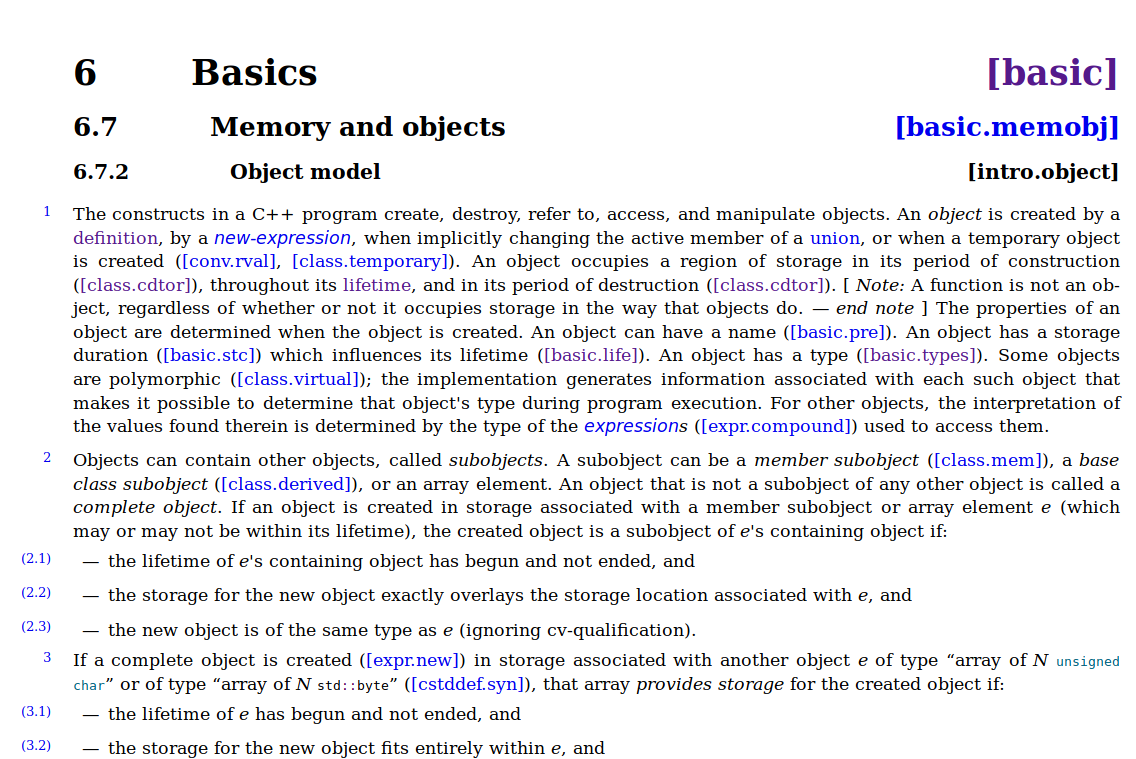
\includegraphics[width=1.0\linewidth]{graphics/objects_basics.png}

\end{frame}


\section{What does the title mean?}

\begin{frame}{Title decomposition}

\centerline{What's the \only{lifetime}<1>\only{\alert{lifetime}}<2-> of your \only{object}<1-2>\only{\alert{object}}<3>?}
\pause
\begin{itemizeSeq}
	\item What is a lifetime?
	\item What is an object?
\end{itemizeSeq}

\end{frame}

\section*{Objects}

\begin{frame}{The object}

Objects are:
\begin{itemize}
	\item created
	\item destroyed
	\item refered to
	\item accessed
	\item manipulated
\end{itemize}

\end{frame}

\begin{frame}{The Object}

\begin{columns}[T]
	\begin{column}{0.58\linewidth}
	
	Is created:
	\begin{itemizeSeq}
		\item by the definition
		\item by the new expression
		\item when changing active\\ member of a union
		\item by creation of the temporary
	\end{itemizeSeq}
	\end{column}

	\begin{column}{0.48\linewidth}
	
	\only{\centering\inputminted{\myCpp}{examples/object-definition.cpp}}<1>
	\only{\centering\inputminted{\myCpp}{examples/new-expression.cpp}}<2>
	\only{\centering\inputminted{\myCpp}{examples/union-active-member-change.cpp}}<3>
	\only{\centering\inputminted{\myCpp}{examples/temporary-creation.cpp}}<4>
	\end{column}
\end{columns}


\end{frame}

\begin{frame}{The object}

Has:
\begin{itemizeSeq}
	\item optional name
	\item storage and it's duration
	\item lifetime
	\item type
\end{itemizeSeq}

\end{frame}

\begin{frame}{The object}

\centerline{Is not a reference {\scriptsize(although reference has lifetime)}}

\end{frame}

\begin{frame}{The variable}

\centerline{Can be either an object or the reference. \pause\alert{Is introduced by a declaration.}}

\end{frame}

\begin{frame}{Summary: variable, reference, object}
\centering
\begin{figure}
\resizebox{0.9\linewidth}{!}{
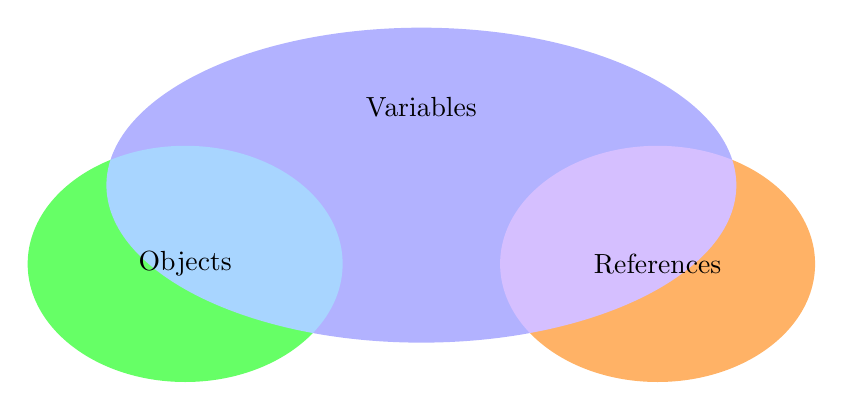
\begin{tikzpicture}
\begin{scope}[blend group=soft light]

\fill[blue!30!white] (0,0) circle[x radius=4cm, y radius=2cm];
\fill[green!60!white] (-3,-1) circle[x radius=2cm, y radius=1.5cm];
\fill[orange!60!white] (3,-1) circle[x radius=2cm, y radius=1.5cm];

\end{scope}

\node at(0,1){Variables};
\node at(3,-1){References};
\node at(-3,-1){Objects};

\end{tikzpicture}}

\end{figure}

\end{frame}


\begin{frame}{Summary: variable, reference, object}
	Just in case you want to check validity with the \href{http://cppreference.com}{\alert{cppreference}}:

	\begin{itemizeSeq}
		\item The object has been recently updated.
		\item The variable definition is unmaintained and unsupported.
		\item Same about references...
	\end{itemizeSeq}
\end{frame}

\section*{Lifetime}

\begin{frame}{What is a lifetime?}

\centerline{Lifetime is a \alert{runtime} property of an object.}

\vfill
\centering

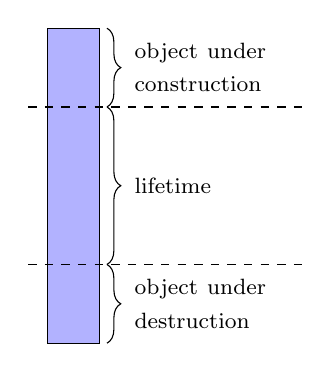
\begin{tikzpicture}

\draw[fill=blue!30!white] (-.75, -2) rectangle (-0.1, 2);

\draw[dashed] (-1, 1) -- (2.5, 1);
\draw[dashed] (-1, -1) -- (2.5, -1);

\draw [decorate, decoration={brace, amplitude=5pt}] (0, 2) -- (0, 1) node[xshift=1.35cm ,midway, text width=2cm]{\footnotesize object under construction};
\draw [decorate, decoration={brace, amplitude=5pt}] (0, 1) -- (0,-1) node[xshift=1.35cm ,midway, text width=2cm]{\footnotesize lifetime};
\draw [decorate, decoration={brace, amplitude=5pt}] (0, -1) -- (0, -2) node[xshift=1.35cm ,midway, text width=2cm]{\footnotesize object under destruction};;

\end{tikzpicture}
\end{frame}

\begin{frame}{What is lifetime?}

\centerline{During the lifetime of an object you can use it without additional restrictions.}

\end{frame}


\begin{frame}{When the lifetime starts}

\centerline{The lifetime of an object starts, when:}

\begin{itemizeSeq}

\item storage with the proper alignment and size for type T is obtained
\item its initialization \alert{(if any)} is complete
\item if the object is a union member or subobject thereof, its lifetime only begins if that union member is the initialized member

\end{itemizeSeq}
\end{frame}

\begin{frame}{Vacuous initialization and trivial types}

You need to create a variable, even if you do not think so (additional copy)

\end{frame}

\begin{frame}{How to fix above}

Richard's changes to the implicit object creation.

\end{frame}


\end{document}